%!TEX TS-program = XeLaTeX
\documentclass[12pt]{article}
\usepackage[top=1in, bottom=1in, left=1in, right=1in]{geometry}

%%%
%% Needed for fonts in xelatex to work
%%%
% NOTE: I actually use XeLaTeX, which allows me to get the fonts
% exactly the way that I want them. For proposals, this means
% I can use Times New Roman instead of the default Computer
% Modern. I actually like Computer Modern, but since Arial
% is what the solicitation suggests there's no point in throwing off a reviewer
% with an unexpected font, particularly one with such a
% polarizing reaction in readers. Never upset the reviewrers, I
% always say.
%
% What's the point of this bit of rambling? If you do not want to use
% XeLaTeX and would rather stick to good old LaTeX, then you
% need to comment out the next few lines of font packages and
% font commands.
%
% If you want to use XeLaTeX but want different fonts, then you
% just need to change the name in the argument for \setmainfont.
% Make sure that the font you use is loaded on
% your machine and your TeX distribution knows how to find it.
% See Google if you need to learn more about this.
%
\usepackage{fontspec}
\setmainfont{Arial}

%%%
%% Packages that I use on a regular basis.
%%%
% Of course, you are likely to need some math typesetting so these
% three packages have you covered.
\usepackage{amssymb}
\usepackage{amsmath}
\usepackage{latexsym}
% I use color, graphicx, and epstopdf to read in PDFs for my figures.
\usepackage{color}
\usepackage{graphicx}
% \usepackage{epstopdf}
% I don't remember why threeparttable and setspace is here. Inertia.
\usepackage{threeparttable}
\usepackage{setspace}
% \doublespacing
%%%
%% Some packages to handle the figures and captions
%%%
\usepackage[labelfont=bf]{caption}
\usepackage{subcaption}
\usepackage{wrapfig}

%%%
%% Packages and settings for my bibliography.
%%%
% apa_with_doi is a style I created to keep DOI in the bibliography
% but strip out URLs. There are a lot of other styles you can
% find for natbib. Again, Google is your friend.
% Author name and year references, i.e., Author (year):
%\usepackage{natbib}
%\bibliographystyle{apa_with_doi}
% Numbered references:
\usepackage[numbers,super]{natbib}
\bibliographystyle{unsrtnat}


%%%
%% Packages and commands to build my table of contents (TOC).
%%%
%% The trick was getting the References included properly.
%% Also, some of my table of contents entry have no page number
%% because those pages are generated separately by my institute.
%% Nothing to be done about that. You may or may not have the
%% same problem, so you may or may not have to tweak this.
\usepackage[nottoc,numbib]{tocbibind}
\renewcommand{\tocbibname}{References}
\usepackage{tocloft}
\renewcommand{\cftsecleader}{\cftdotfill{\cftdotsep}}

%%%
%% These commands get the spacing around the title and section titles right.
%%%
% I tightened up the spacing. The LaTeX default is just too roomy.
% This spacing is still clean and legible, just not so free with the
% whitespace between sections.
%
% First the title.
\usepackage{titling}
\setlength{\droptitle}{-50pt}
\pretitle{\begin{center}\Large\bfseries\vspace{0ex}}%
\posttitle{\end{center}\Large\vspace{-2ex}}%
\preauthor{\begin{center}\large}%
\postauthor{\end{center}\large\vspace{-3ex}}%
\predate{\begin{center}\large}%q
\postdate{\end{center}\large\vspace{-6ex}}%
% Now the section headings.
\usepackage[noindentafter]{titlesec}
\titleformat{\section}{\large\bfseries}{\thesection}{1em}{}
\titlespacing{\section}{0pt}{18pt plus 2pt minus 2pt}{4pt plus 2pt minus 2pt}[0pt]
\titlespacing{\subsection}{0pt}{16pt plus 2pt minus 2pt}{4pt plus 2pt minus 2pt}[0pt]
\titlespacing{\subsubsection}{0pt}{14pt plus 2pt minus 2pt}{4pt plus 2pt minus 2pt}[0pt]

%%%
%% These commands get the lists to work the way that I want them to.
%%%
% i.e. I want less space wrapping around the list.
\usepackage{enumitem}
\setlist{nolistsep}
\setlist[2]{noitemsep}
\setlist[1]{noitemsep}

%%%
%% Commands for making the tables.
%%%
\usepackage{booktabs}
\usepackage{multirow}
\usepackage{array}


%%%
%%% Formatting urls
%%%
\usepackage{url}
\urlstyle{rm}

%% The lineno packages adds line numbers. Start line numbering with
%% \begin{linenumbers}, end it with \end{linenumbers}. Or switch it on
%% for the whole article with \linenumbers after \end{frontmatter}.
\usepackage{lineno}

%% In order to have a caption to the side of a figure or table, use the
%% 'sidecap' package.
\usepackage[rightcaption]{sidecap}
\sidecaptionvpos{figure}{t}

\usepackage{wrapfig}


%% For more control of the enumeration environment (lists with numbers)
%% use the enumitem package.
%\usepackage{enumitem}

%% Also, to reset the numbering of enumerate, use the following:
%\setenumerate[0]{label=\alph*.}

% To deal with figures all alone on a page.
\renewcommand{\floatpagefraction}{.8}%

% To use symbols for the footnotes:
\renewcommand{\thefootnote}{\fnsymbol{footnote}}

% set up the page numbers as 1-N, 2-N, ...
\numberwithin{page}{section}
\renewcommand{\thepage}{\thesection-\arabic{page}}

% https://tex.stackexchange.com/questions/210871/latex-page-numbering-by-section
%this does not seem to work, just hard code it :(
% not sure if there is something else in this template that is breaking it
% or things have changed in the last 6 years?
%\usepackage{etoolbox}
%\makeatletter
%% Make sure that page starts from 1 with every \section
%\patchcmd{\@sect}% <cmd>
%  {\protected@edef}% <search>
%  {\def\arg{#1}\def\arg@{section}%
%   \ifx\arg\arg@\stepcounter{page}\fi%
%   \protected@edef}% <replace>
%  {}{}% <success><failure>
%\makeatother

%% Finally, we get to the document.
\begin{document}
\title{Improving the Foundations and Maintenance of Matplotlib and CartoPy}
\author{Dr. Thomas A Caswell\\Dr. Ryan May}
\date{}
\maketitle

% First, let's get that TOC in there. NASA likes it.
\setcounter{tocdepth}{2}
\tableofcontents
\thispagestyle{empty}
% Let's leave this TOC alone on this page and start a new one for
% proposal body.
\newpage

\section{Scientific/Technical/Management (S/T/M)}
% Let's reset the page counter.
\setcounter{page}{1}
% the subsection are a combination of the lines labeled "Content" in
% Table 1 (on ROSES-20 SoS-51) and the text in E.7.3 (on E.7-2 -
% E.7-3) describing what needs to be in the proposal.

% not sure that this order is right, but I think we need to hit all of
% these points.  Maybe want to rename the section headings or merge
% some of them?
\subsection{description of software and relevance to SMD}

Billions of dollars of SMD funding, across all 4 SMD divisions,
critically relies on the scientific Python ecosystem (SPE) for data
analysis, scientific computation and visualization.  This includes
flagship missions like Hubble, JWST, and the Curiosity Rover.  The
Scientific Python Ecosystem is a loosely defined community of projects
and programmers with the common goal of advancing Science through the
use of the Python programming language.  This development is largely
volunteer work, or work that is sponsored implicitly by specific
science projects.  SPE, shown with a rough schematic in Figure
\ref{fig:ecosystem}, has a core of general purpose domain-agnostic
tools, like NumPy\cite{Harris2020} and SciPy\cite{Virtanen2020}, with
concentric rings of increasingly domain specific tools, like
AstroPy\cite{robitaille2013astropy} and
SunPy\cite{sunpy_community2020}, extending the core.
Matplotlib\cite{Hunter:2007} is the fundamental data visualization
library for the SPE. This layered approach gives scientists and
engineers convenient high level tools while enabling direct access to
the underlying libraries when needed.



\begin{wrapfigure}{r}{0.5\textwidth}
  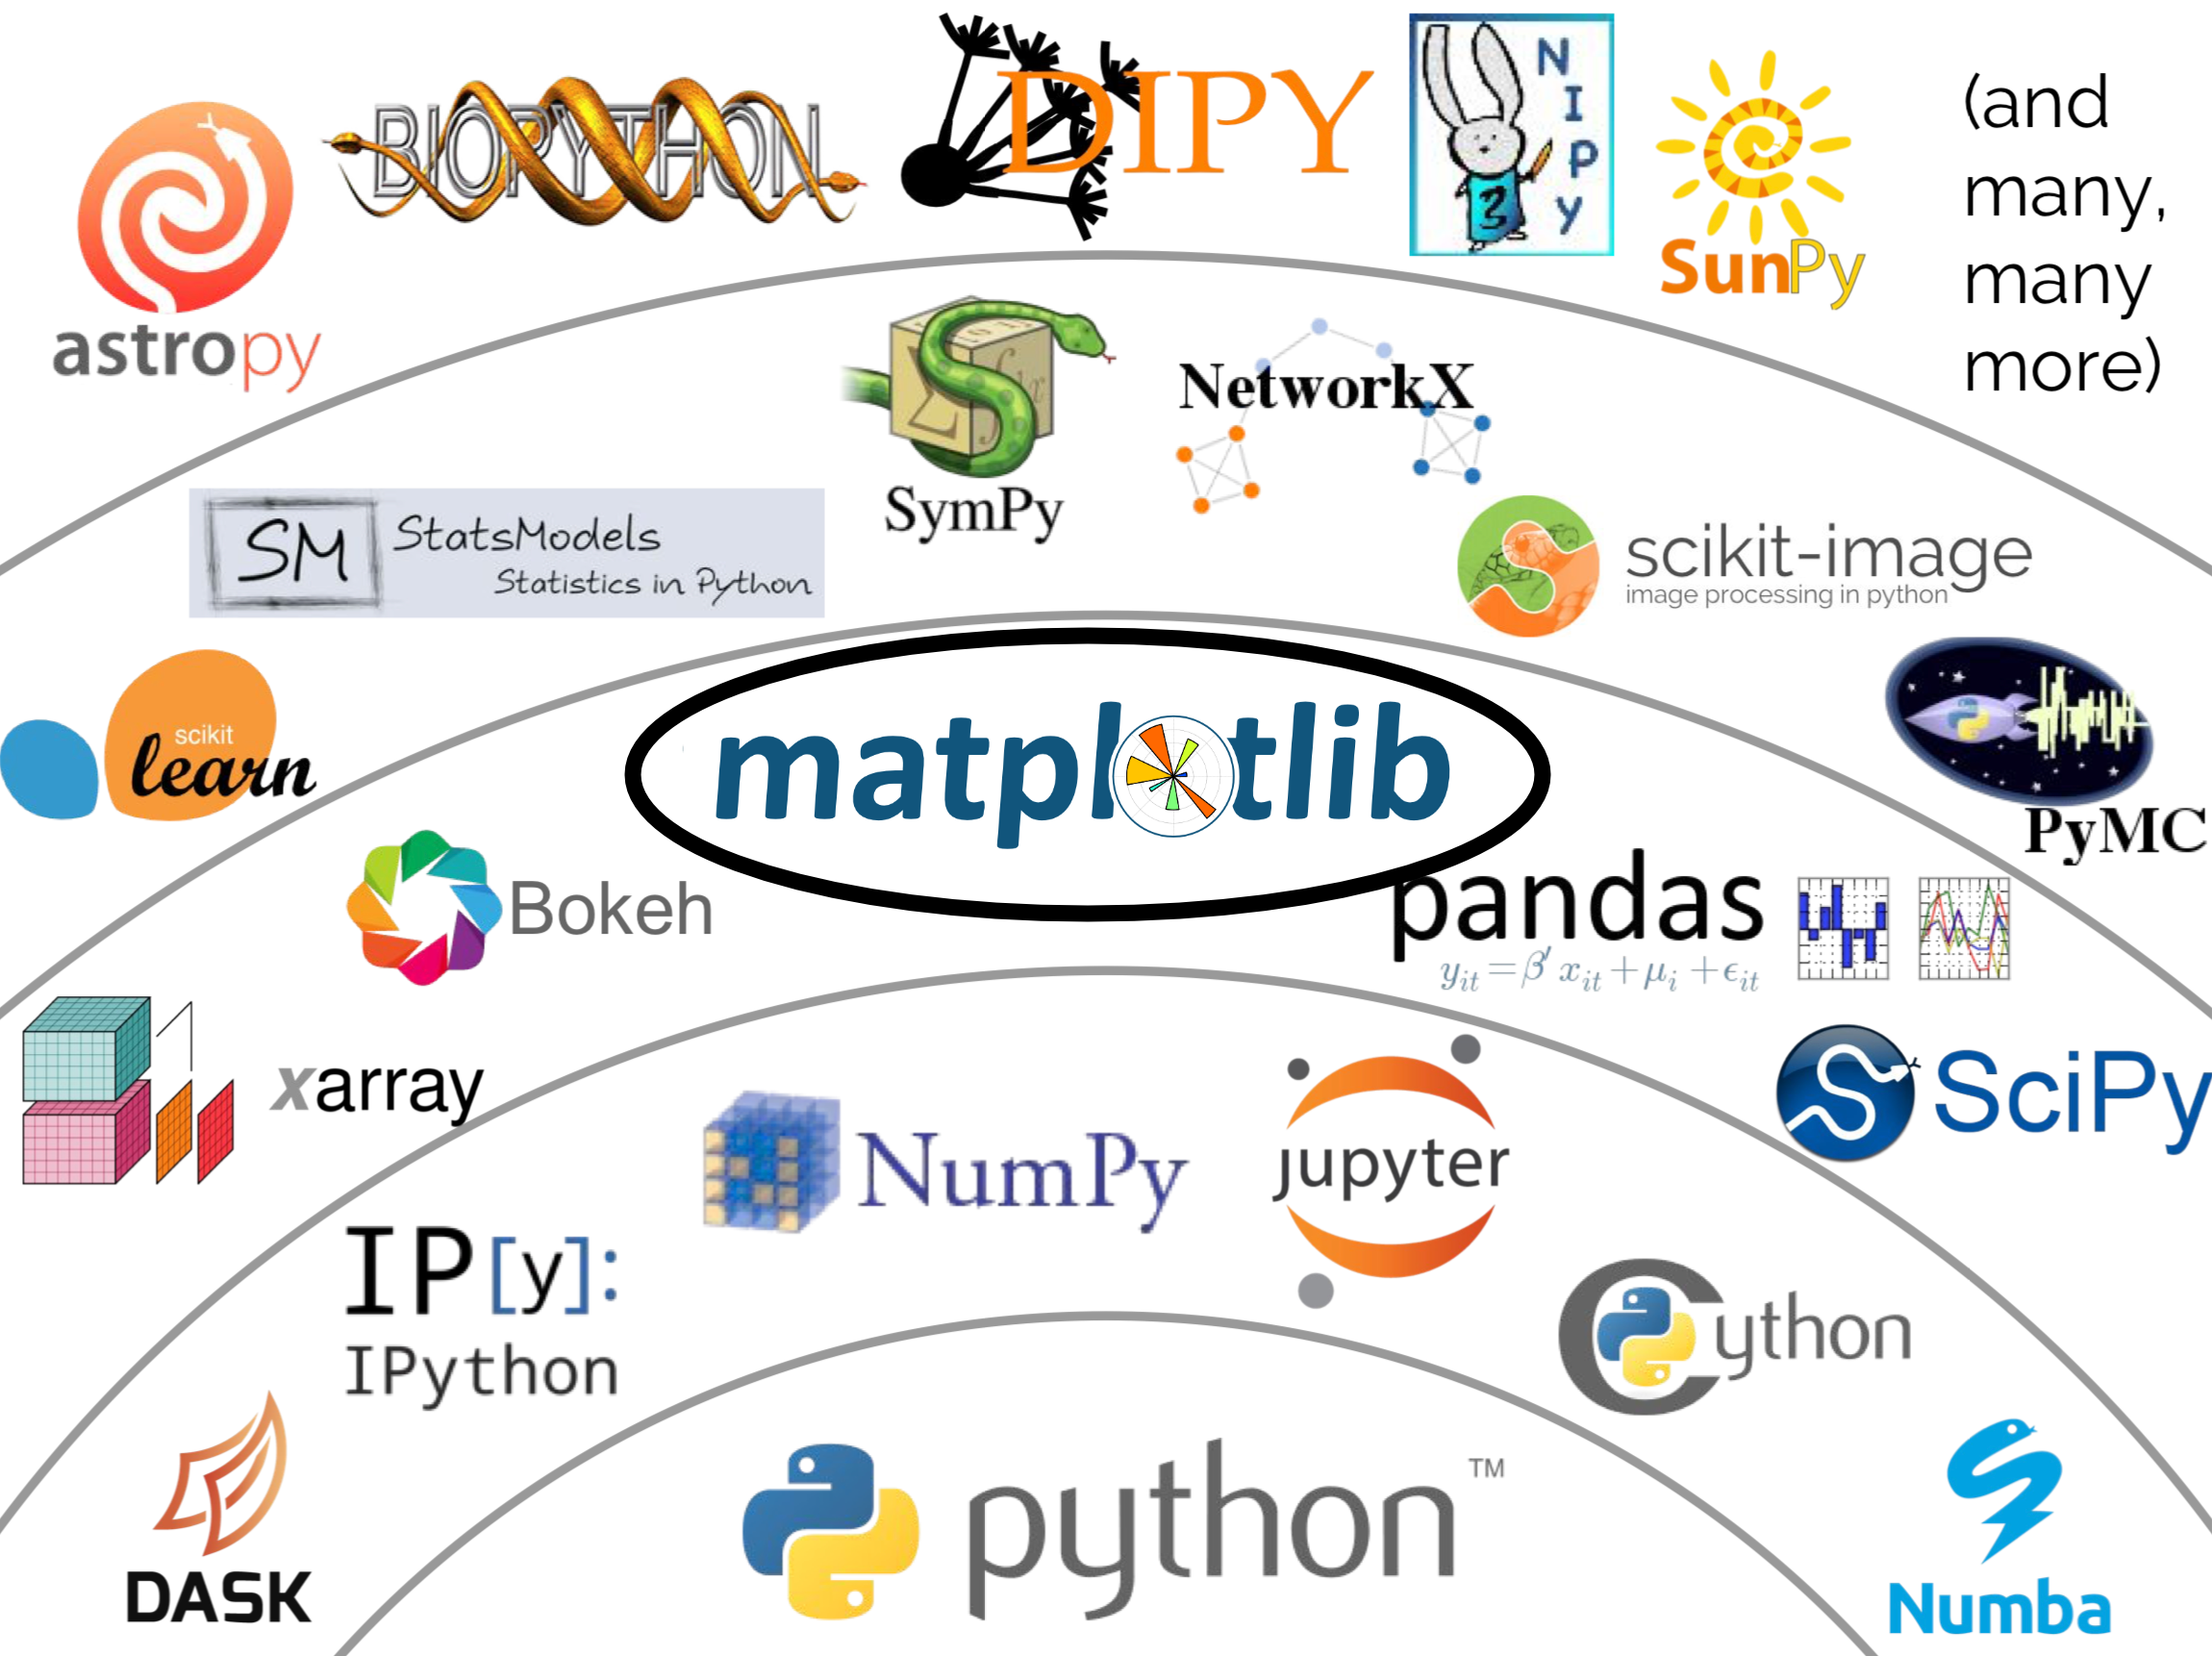
\includegraphics[width=0.45\textwidth]{scipy-ecosystem}
  \caption{A schematic of the Scientific Python ecossytem.  At the
    center we have the Python language itself with concentric rings of
    domain agnostic to domain specific libraries.  Both AstroPy (top
    left) and SunPy (top right), used in the astrophysics and
    heliophysics divisions respectively, rely on Matplotlib. Cartopy,
    which is not shown, would be placed in the outer [CHECK] ring.
    Credit: Jake van der Plas, "The Unexpected Effectiveness of Python
    in Science", PyCon 2017}
  \label{fig:ecosystem}
\end{wrapfigure}



Matplotlib \cite{Hunter:2007} is an established open source plotting
library with a BSD-derived license that is currently used through out
both the SMD science community and the wider scientific community.
The initial commits in the Matplotlib history date to early 2003 and
the initial work was done in 2001-2002. Matplotlib has been actively
developed and maintained by a vibrant, primarily volunteer, community
over the last 17 years.  Matplotlib has over 1,300 individual
contributors to the code base, is in top 100 most downloaded Python
packages from pypi, and is packaged by every major linux distribution.
Matplotlib has an API for both quick plotting, as required from
exploratory data analysis, a low-level API that gives full control the
visualization for fine-tuning plots for publication, tools to write
GUI independent interactive data exploration tools, animation support,
and the ability to write out to a variety of vector and raster
formats.

The most common visualizations in a domain need to be fluid for the
end-practitioners, with the ``obvious'' customization options
exposed. Much of the domain-specific specialization is carried in the
structure, semantics and assumptions of the data, and in the standard
visualizations of the domain. These specializations can vary widely,
in contradictory ways, between domains. Because no high-level API can
simultaneously satisfy all of the visualization needs, there has
developed a rich ecosystem of domain specific plotting tools including
including yt, astropy, ArviZ, xarray, cartopy, astropy,
fast\_histogram, CartoPy, and metpy [tune to be more NASA specific?].


CartoPy is a Matplotlib extension library that brings support for
mapping applications to Matplotlib, providing support for plotting
using a variety of map projections (both terrestrial and non) as well
as providing out-of-the-box support for many terrestrial map
features. CartoPy is currently the only Matplotlib-based plotting
library for mapping applications being actively developed in the
Python ecosystem. CartoPy is frequently used for earth science
applications, including many uses of NASA Earth science datasets [TODO cites].


While large parts of the scientific computing community rely on the
SPE, the open nature of these infrastructure tools makes measuring
their influence hard.  Conservative estimates, based on downloads and
web traffic on the documentation, are that Matplotlib has over a
million users.  We expect that a large fraction of NASA SMD-sponsored
projects rely on this shared infrastructure to some degree, but this
is hard to prove in practice.  In particular, scientific work does not
usually cite the software that was used for computation, and usage and
download statistics are hard to gather for widely used open source
packages.  Even though citation counts are likely to vastly
under-represent the scientific use of these packages,
Matplotlib~\cite{Hunter:2007} over 6000 citations while a common
reference of NumPy\cite{walt2011numpy} has over 3200 citations [TODO
  update the citation counts]. These counts already illustrate a
problem in measuring usage using citations, as every user of
Matplotlib also uses NumPy, but Matplotlib has twice as many
citations.  Domain specific tools, like
AstroPy~\cite{robitaille2013astropy} for astronomy (about 2000
citations) often have high citation counts compared to the core
packages like NumPy, SciPy and Matplotlib that they are built upon.


\subsection{Objectives and Significance}
We propose a three prongs of work:
\begin{itemize}
\item Fully Document, test, and fix existing unit handling code in Matplotlib.
\item Overhaul how cartopy binds to PROJ and GEOS
\item General maintenance of Matplotlib and cartopy
\end{itemize}
These tasks are ill suited to volunteer work: they either require
significant dedicated effort or simply do not attract volunteer
effort.  The first two tasks will likely require a large fraction of
an FTE and need long blocks of un-interrupted work time to complete.
Maintenance is inherently reactive, we do not know about new bugs,
user issues, or breaking changes in upstream packages until they are
reported to us.  Many of our volunteers are fixing a bugs or
implementing a features that they affect them personally which
provides an inherent motivation..  While this critical work can be
done by volunteers, if we want to commit to a service level we need
paid developer time.


\subsubsection{Cartopy guts}
CartoPy's mapping capabilities leverages the widely-used PROJ library
for mapping projections and the GEOS library for geometry
applications. Currently, CartoPy maintains custom code to interface
Python with these C-based libraries. As part of this work, we propose
porting Cartopy to instead use existing libraries that provide Python
bindings for these libraries, PyPROJ and PyGEOS. Not only will this
reduce CartoPy's overall amount of code and enhance maintainability,
but it will also address two of the biggest challenges that occur in
packaging CartoPy for its user-base.


\subsubsection{Unit work}

Units are fundamental to science, however most numerical software is
unit-naive.  It the user's responsibility to keep track of and
correctly convert data to commensurate units prior to any computation.
Failing to do so leads to the most insidious of bugs: everything
``works'' but silently gives the wrong answer.  Matplotlib supports
their use for unit-aware plotting using any of the high-level
libraries for unit-aware data structures in Python.  The initial
development of this capability was supported by NASA and it is
currently used to support spaceflight operations by Monte, JPL's
mission design and navigation software system.

However, this support is under documented making it difficult for
users to understand how to fully make use of the capability and for
developers to extend it.  Further, because we do not have full test
coverage of all plotting functions to verify that they correctly
handle units we have had a number of regressions in the functionality.
We will propose to write thorough user and technical guides to working
with unit-aware data in Matplotlib, add 100\% test coverage of unit
support in our plotting routines, and fix any issues and
inconsistencies discovered in this process.  Once we have hardened the
existing functionality to make working with unit-full data easier.

If Matplotlib detects units on user input then we look up the correct
conversion function to map to unit-naive values we need internally and
the configure the Axis to place ticks and format the tick labels
correctly.  By default Matplotlib registers a converters for time and
string-categorical data. Users and third-party libraries can register
their data structures and converters at run time to extend this
dispatch mechanism.

The first task is to document the full details, both at the conceptual
and API level, how the unit dispatch system works in theory and how it
works in practice.  This documentation will be aimed at Matplotlib and
third-party library developers that want to use and extend the unit
system.  The original authors of the unit code are no longer active
with the project so we may have to reverse engineer some aspects.
Understanding and documenting the current state of the library and how
it was intended to work will be the foundation of the rest of the
work.

The second task is to write several user-facing tutorials making use
of the unit-full types we support by default and commonly used
down-stream unit libraries such as
\texttt{unyt} (\url{https://unyt.readthedocs.io/en/stable/})
and
\texttt{pint} (\url{https://pint.readthedocs.io/en/stable/}).
In parallel we will reach out to the community to find any additional
users, such as the Monte developers, who depend on the unit machinery
to make sure that the examples are representative of how they actually
use the functionality.  As with the developer documentation this will
serve as foundation for the rest of the work, however this
documentation may be prescriptive of the behavior we want to have
rather than the currently implemented behavior.

The third task is to ensure that all of the plotting methods support
unit-full data in a uniform way.  This should include handling units
on the initially passed, if the data is updated, and changing the
displayed units.  We will address known bugs and inconsistencies, and
expect to find additional bugs that will need to be addressed.  The
documentation developed as part of the first two tasks will guide how
we resolve any inconsistencies.  Fixing these issues may require
significant refactoring of the internal representation of the
un-converted and converted data; this work will likely compliment and
build on the ongoing work to refactor the Artist and data storage
layers.

A final task is to extend the unit machinery to improve the user
experience.  Currently much of the mechanism of unit-handling is
implicit and automatic based on type inference.  We propose to extend
the interface to allow optional direct control of the unit machinery
by users and third-party library developers.  We will rely on the
documentation and testing from the previous work to ensure that we do
not introduce any new regressions or inconsistencies.



\subsubsection{General maintenance}

Matplotlib and Cartopy are community-driven projects, but we have
grown to the point where we need developers with the time to organize,
plan, and make decisions.

To maintain Matplotlib's and Cartopy's health we need to:
\begin{itemize}[noitemsep]
\item fix critical bugs and regressions;
\item triage the backlog of Issues and PRs in terms of topic,
  difficulty, and urgency and promptly triage newly opened Issues and
  PRs;
\item maintain backward compatibility and extensively document
  intentional changes;
\item on-board new contributors to sustain and diversify developer
  team;
\item and manage discussions about proposed enhancements, features,
  and API changes.
\end{itemize}
The requested support for developers is intended to complement and
facilitate, not replace, crucial volunteer work.  We aim to better
co-ordinate and nurture their efforts, with the goal of growing and
sustaining a diverse community of volunteer and paid expert
contributors.


Pull Requests (PRs) and Issues are submitted faster than they can be
reviewed; Matplotlib has accumulated about 300 open PRs 1300 open
Issues due to this imbalance, while CartoPy currently stands at 40
open PRs and 229 open Issues.  This imbalance is not due lack of
activity, in 2020 Matplotlib resolved 125-200 PRs and 75-125 Issues a
month but only reduced the PR backlog by 70 open PRs and made no
progress on reducing the Issue backlog.

There may be critical bug reports or insightful feature requests among
the issue backlog, while among the PR backlog are useful contributions
or bug fixes that would improve the libraries for direct users and
downstream packages.  The large backlog is discouraging for new and
occasional contributors and distracting for core developers.  The
resources we will request will help to significantly reduce, but not
eliminate, this backlog.


For 10 months in 2020 we had a full time RSE working on Matplotlib who
had a measurable impact on both the rate of PR review, the rate of
issue resolution, and fixed a number of long standing bugs.  He has
had the time and bandwidth to address a number of long-standing issues
such as [TODO highlights from Elliott].

There are a number of unglamorous tasks that are required to ``keep
the lights on'' on a Python package include things like maintaining
the CI, release management, tracking down platform specific bugs.
These are tasks that are never ``done'', as users find new ways to use
the library which require new features or as the world changes around
us.

\subsection{Perceived impact of work}
\begin{enumerate}
\item increased reliability of unit-aware plotting
\item improvement in general reliability of software
\item improved responsively to issues
\item easier installation and deployment
\end{enumerate}
\subsection{Relevance to program element}

TODO make this flow...at all...

Matplotlib is used through out all of the program elements of the SMD.
In Earth observation Matplotlib has been used to study thunderstorms
\cite{https://doi.org/10.1002/2016JD025299,https://doi.org/10.1029/2019JD030874},
seasonal ocean winds \cite{https://doi.org/10.1002/2017JD027516} and
tropical storms \cite{Lang_2020}.  Matplotlib was used in the first
science paper from the Parker Solar probe\cite{Bale2019}.  Matplotlib
has been used as part of the Martian science program in both an
orbiter \cite{https://doi.org/10.1029/2019JE006188} and
rover\cite{https://doi.org/10.1002/2016EA000219} contexts.
Historically, Matplotlib was used as part of ground operations from
the Phoenix Lander.  Matplotlib was used on data from Kepler and K2
missions to study Trojan asteroids\cite{Nixon_2019} and Titan
\cite{Ryan_2017,2019PASP..131h4505P}.
Matplotlib is used for visualization of scheduling, safety+constraint checks, and telemetry by the Swift science operations team \cite{swift_ops,2020ApJ...900...35T}.
Both the Hubble and James Web Space Telescopes data processing
developed by Space Telescope Science Institute rely on Matplotlib [CITE NEEDED].
Matplotlib is used to support spaceflight operations by Monte, JPL's
mission design and navigation software system [CITE NEEDED].
Matplotlib is being used in the New Horizons Kuiper belt extended mission \cite{Porter_2018}.  Matplotlib
has been used for fundamental research on graphene \cite{PhysRevLett.120.236802} and
work on nuclear rockets \cite{leu_cerment}.

Need more examples of SMD using Cartopy!

Matplotlib supports plotting unit-aware data structures which have
been used to support spaceflight operations by Monte, JPL's mission
design and navigation software system. (TODO expand this!)

\subsection{Technical approach and methodology}

our standard practice!

\subsection{sources of uncertainty/mitigation to risk}

The biggest risk with the proposed work is that we are underestimating
the amount of work that will be required for both the unit work and
the CartoPy refactoring.  Particularly with Matplotlib, there is the
risk that when you start to pull on a thread the scope of work rapidly
snow balls as there can be unexpected internal dependencies or edge
cases that are not apparent at first glance but must be accounted for.
However, by working incrementally we can ensure that any effort
applied has a positive benefit, if less than initially planned.  In a
worst case where we have to abandon the work we will maintain the
status quo.

We anticipate that all the work can be done incrementally and will be
merged to the default branch of Matplotlib throughout the performance
period.  This necessary because, as a community project, any work that
goes in needs to go through the same review process.  Many smaller PRs
are much easier to review than a single huge PR.  This process in turn
inherently reduces the risk of this work as we will be continuously
merging any progress made to the default branch.  These improvements,
both to the code and documentation, will be released to users as part
of our standard 6mo release cadence.

Maintenance is extremely low risk.  There is large volume of
individually small tasks that need to be addressed: the issue and PR backlogs.
Any dedicated effort devoted to clearing the backlog will meaningfully improve
both libraries.

[section on effect of having an RSE]

\subsection{roles of team members}
\begin{enumerate}
\item RSE: maintenance + lead unit unit testing (1FTE)
\item May: Cartopy refactor + unit expertise + maintenance (0.25FTE)
\item Caswell: PI + maintenance + community/governance work (0.1FTE)
\end{enumerate}

\subsection{workplan with milestones}


Starting from July 2021 onward Dr. Caswell will devote 10\% FTE to
this work.  This time will be split between managementand Matplotlib
maintenance.  Both of these are on-going tasks.  This will supplement
separately funded 30\% FTE from Dr. Caswell on Matplotlib related work
through 2021.  The first task will be the recruitment and hiring of
the RSE.

The Research Software Engineer, whom needs to be identified, will
devote 100\% FTE to this project.  This will be split evenly with 50\%
FTE being spent on the unit work and 50\% being spent on maintenance
of Matplotlib and Cartopy until the unit work is complete.  If the
unit work is completed faster than expected, the RSE will devote 100\%
of their effort to Matplotlib and Cartopy maintenance.  Because
Matplotlib is a community project, the work of the RSE will still go
through the normal review process.  The interaction with community
makes it advantageous to spread out the unit work.  The first task,
producing developer-facing documentation about how the unit system
works we expect to take 20\% FTE with will be spread across the first
6mo of the grant.  Similarly, writing the user-facing documentation
should take about 25\% FTE which will be done is the 7-12mos of the
performance period.  The remaining work on units, adding the tests,
fixing any bugs and inconsistencies, and any required internal
refactoring, will take 1 FTE and will be spread across final 2 years
of the performance period.  Incremental progress will be merged and
released as part of the normal release cycle throughout the
performance period.  The RSE will present the status of the work at
two conferences, expected to be SciPy in July and one of PyData
conferences in the winter.


\begin{description}

\item[Y1Q1] Begin first units task (documenting current behavior)
\item[Y1Q2] Finish first task. Have developer documentation merged to
  Matplotlib docs.
\item[Y1Q3] Begin second task.
\item[Y1Q4] Finish second task. Have user-facing documentation merged
  to Matplotlib docs. Present at SciPy and/or pydata.

\item[Y2Q1] Begin third task.  Develop detailed development plan.
\item[Y2Q2] Continue third task.
\item[Y2Q3] Continue third task.
\item[Y2Q4] Present at SciPy and/or pydata.


\item[Y3Q1] Continue third task. Evaluate progress on development
  plan, adjust if needed.
\item[Y3Q2] Continue third task.
\item[Y3Q3] Continue third task.
\item[Y3Q4] Completed third task. Present at SciPy and/or pydata.

\end{description}

From July 2021 onward Dr. May will devote 25\% FTE to this work.  That
effort will be split between overhauling the CartoPy binding to PROJ
and GEOS, providing technical assistance to the RSE for the unit work,
and general maintenance of both Matplotlib and Cartopy.


\begin{description}

\item[Y1Q1]
\item[Y1Q2]
\item[Y1Q3]
\item[Y1Q4]

\item[Y2Q1]
\item[Y2Q2]
\item[Y2Q3]
\item[Y2Q4]


\item[Y3Q1]
\item[Y3Q2]
\item[Y3Q3]
\item[Y3Q4]

\end{description}


\subsubsection{Grant Management Plan}

Dr. Caswell of BNL is the PI of the proposed development and is.  the
Matplotlib Lead Developer.  He is responsible for the quality and
direction of the proposed work and the proper use of all awarded
funds.  He is also responsible for all management, and budget issues
and is the final authority for this task.

Dr. May is responsible for the quality and direction of the work as
related to Cartopy.

Dr. Caswell and Dr. May will share responsibility of supervising the
RSE.




\subsection{Project Management}
\subsubsection{Governance}
Matplotlib is a NumFOCUS Fiscally Sponsored Project.  The governance
is specified at
\url{https://github.com/matplotlib/governance/blob/master/governance.md}.
The project has a Project Lead (Caswell) who is the final authority in
all decisions, however when possible all decisions are made by
community consensus.  In addition to the Project Lead, there is a
formalized Steering Council which is responsible for the overall
direction of the project, and several Deputy Project Leads who have
day-to-day technical responsibilities.

TODO need to cover history of project lead changing



\subsubsection{License}

BSD-derived and LGPL

\subsubsection{sustainability metrics}
\begin{enumerate}
\item Continue Regular releases (mpl minor every 6mo, patch every 2mo
  or as needed).
\item Increase number of new regular contributors
\item Rate of PR / Issue throughput
  \begin{enumerate}
  \item caveats on how issues/PRs are very varied in time to resolve
  \end{enumerate}
\end{enumerate}

\subsubsection{collaboration with related projects}

None of the projects in the Scientific Python ecosystem existing in a
vacuum; most users use more than one of the projects.  While developer
communities exist around each of the code bases, there is also a
broader community across the projects.  Matplotlib developers are part
of this community and Matplotlib developers have well established
relationships with the other projects in the ecosystem, including our
key up and down stream dependencies.

Much of the communication is through the standard communication
channels, such as reporting issues to each other's issue trackers,
asking questions on mailing lists or discussions forums, and
submitting patches.  Additionally, through NumFOCUS and domain
conferences there are regular in-person meetings.

Almost all of the Matplotlib contributors, are domain experts in their
primary domain and use Matplotlib for their research.

The strongest relationships, both historical and current, are with
projects where we have shared developers.  For example Ryan May and
Elliot sales de Andre are both core contributors to Matplotlib and
Cartopy.  Micheal Droettboom, the previous Matplotlib Project lead,
was also a core developer on Astropy.



\subsubsection{inclusive practices}

Matplotlib strives to be an inclusive and open project and have
adopted a Code of Conduct
\url{https://github.com/matplotlib/matplotlib/blob/master/CODE_OF_CONDUCT.md}. Anyone
who is willing to contribute to the project should be able to do.  It
is important for everyone working on the project to feel safe to make
mistakes.

One challenge of being an open community developed project is that we do not
have reliable demographics on a vast majority of our contributors.

We have recently started two efforts to improve the development and
retention of new contributors: an ``incubator'' channel on gitter and
a Triage Team.

The hardest part of getting started to contributing to open source
projects is can be simply getting started.  The incubator is a
semi-closed chat room where new contributors can get support on any
aspect of contributing to Matplotlib.  This include the technical
aspects of the code they are working on, help with git/github, our
review process, or the social expectations and norms of the community.  The
goal is that by providing this support to first time contributors we will
retain more of them as regular contributors and then maintainers.

The issue tracker is important to communication in the project because
it serves as the centralized location for making feature requests,
reporting bugs, identifying major projects to work on, and discussing
priorities.  For this reason, it is important to curate the issue
list, adding labels to issues and closing issues that are resolved or
unresolvable. Triaging issues does not require any particular
expertise in the internals of Matplotlib but is extremely valuable to
the project.  To this end we have created a ``Triage Team'' in the
organization who have power to tag, milestone, and close issues.  In
addition to the direct benefit of improving the issue triage and
freeing the core-developers to spend more time reviewing PRs, this
role will bring more people into the developer community and may
provide a path way to becoming regular contributors and maintainers.


We will work with NumFOCUS to develop metrics and evaluate the efficacy of
these efforts at diversifying our contributor base.

\subsubsection{information dissemination}

As a project Matplotlib maintains a range of communication channels
aimed at several, overlapping, audiences.  This include a weekly
developer call, an active chat room on gitter, issues tracker and PRs
on github, mailing lists, a discourse forum, in-person presentations
at conferences and pydata events, the published documentation
(inculding historical and ``future'' versions), a blog, and several
social media accounts.

The weekly developer calls are typically attended by six to eight
people and are used for high-bandwidth discussions about both the
overall direction of the project and technical issues depending on the
day.  The agenda and minutes are publicly
available (\url{https://hackmd.io/team/matplotlib}) and the
calls are open to all.

Matplotlib has an active
gitter (\url{https://gitter.im/matplotlib/matplotlib}) chat
room.  This is used for real-time chat for general coordination,
resolving small technical issues, and user support.  While the chat
room's history is persistent it is treated as transient.  For more in
depth discussions we try to move the conversation to either the issue
tracker, for bug reports and PR discussions, or discourse, for user
support.

The center of gravity of Matplotlib development takes place on
GitHub (\url{https://github.com/matplotlib/matplotlib}) via
Issues and PRs.  We try to keep the discussions on GitHub restricted
to bug reports, feature requests, and discussions about the code in
PRs.  In addition to the source, the official documentation is hosted
in the same repository.  Our governance is tracked in a different
repository, also on
GitHub (\url{https://github.com/matplotlib/governance}).

For user support and more general discussion we maintain a mailing
list (\url{https://mail.python.org/mailman/listinfo/matplotlib-users})
and a discourse (\url{https://discourse.matplotlib.org})
instance.  While users have to subscribe and register respectively,
these forums are open to all.

When we could travel Matplotlib developers would frequently attend
in-person meetings including SciPy and PyData events.

We publish extensive prose, example, and API
documentation (\url{https://matplotilb.org}) that is
refreshed with each release.  In addition to the top-level docs, which
always refer to the most recent release, we also host historical and
development versions of the documentation.  We have between 700k-1M
unique visitors a month to the documentation.

We have a blog (\url{https://matplotlib.org/matplotblog/})
which hosts user-submitted content highlighting work they have done
using Matplotlib.

We have project accounts on several social media platform including
twitter and Instagram.


\subsection{current workflow}

Matplotlib is an established community driven in the ``federation''
model as defined by Nadia Eghbal\cite{eghbal_2020}.  We have a core
group regular maintainers who take responsibility for reviewing and
merging proposed changes to the library.  We strive for consensus and
rely on the judgment of our maintainers.

Matplotlib manages proposing and reviewing contributions to the
library and documentation though a variation on the ``git flow''
process (\url{https://guides.github.com/introduction/flow/})
on GitHub (
\url{https://matplotlib.org/devel/coding_guide.html}).  A contributor,
either one of our core maintainers or a first time contributor, will
open a ``Pull Request'' from their fork of Matplotlib to propose some
change.  Once the PR is opened continuous integration (CI) is
automatically run to preform a variety of regression and style checks.
In parallel the code is reviewed by the maintainers who either request
changes, which starts a cycle of iteration with the contributor, or
approves.  Once consensus is reached the PR is merged and those
changes will be included in the next release.

The threshold for merging a PR depends on the reviewer judgment of the
risk of the changes.  PRs that only change documentation, which can
not introduce regressions or introduce new features, may be merged by
the first reviewer where as all code changes need to be reviewed and
approved by at least two maintainers.  However in either case a
maintainer may wish to leave a positive review but not merge the PR.
If a maintainer objects and requests changes then the PR will not be
merged until those issues have been addressed.  If consensus can not
be reached the default is the status quo (not merging) and the
decision may fall back to the Deputy Project Lead or Project Lead to
break the log jam.

Matplotlib is cautious about making backwards-incompatible change that
intentionally break users existing code.  While in an ideal world,
future versions of the library would always be 100\% backwards
compatible, sometimes we do need to make incompatible changes.  As
part of the review process we check that there if there are any API
changes and if so that they are well justified and documented.  When
technically possible we try to provide user-visible warnings the
version before we actually implement the breaking change.  This gives
us a window of time for users to either adapt to the change or to
communicate to us that they can not adapt so we can reconsider the
change.  Given this high barrier to changing or removing behavior we
are careful to make sure that any new API we add to the library is
well thought out and complete because once we have released a version
of the library with that code it is hard to take it back.  These
considerations together are important enough that we have a Deputy
Project Lead responsible for API consistency.

This process works well for incremental contributions and bug fixes,
new features or bigger changes are typically discussed before
significant work is done.  In many cases if the feature does not need
to be in the core library we encourage contributors to create a new
stand-alone project.  This has several advantages including the giving
the author more control, allows them to iterate faster than our
relatively slow 6 month release schedule, and gives them greater
flexibility to change their API after initial


\newpage
% Here's how I get references.
% needed for AAS citation

\def\ref@jnl#1{{\rm#1}}

\def\aj{\ref@jnl{AJ}}                   % Astronomical Journal
\def\actaa{\ref@jnl{Acta Astron.}}      % Acta Astronomica
\def\araa{\ref@jnl{ARA\&A}}             % Annual Review of Astron and Astrophys
\def\apj{\ref@jnl{ApJ}}                 % Astrophysical Journal
\def\apjl{\ref@jnl{ApJ}}                % Astrophysical Journal, Letters
\def\apjs{\ref@jnl{ApJS}}               % Astrophysical Journal, Supplement
\def\ao{\ref@jnl{Appl.~Opt.}}           % Applied Optics
\def\apss{\ref@jnl{Ap\&SS}}             % Astrophysics and Space Science
\def\aap{\ref@jnl{A\&A}}                % Astronomy and Astrophysics
\def\aapr{\ref@jnl{A\&A~Rev.}}          % Astronomy and Astrophysics Reviews
\def\aaps{\ref@jnl{A\&AS}}              % Astronomy and Astrophysics, Supplement
\def\azh{\ref@jnl{AZh}}                 % Astronomicheskii Zhurnal
\def\baas{\ref@jnl{BAAS}}               % Bulletin of the AAS
\def\bac{\ref@jnl{Bull. astr. Inst. Czechosl.}}
                % Bulletin of the Astronomical Institutes of Czechoslovakia
\def\caa{\ref@jnl{Chinese Astron. Astrophys.}}
                % Chinese Astronomy and Astrophysics
\def\cjaa{\ref@jnl{Chinese J. Astron. Astrophys.}}
                % Chinese Journal of Astronomy and Astrophysics
\def\icarus{\ref@jnl{Icarus}}           % Icarus
\def\jcap{\ref@jnl{J. Cosmology Astropart. Phys.}}
                % Journal of Cosmology and Astroparticle Physics
\def\jrasc{\ref@jnl{JRASC}}             % Journal of the RAS of Canada
\def\memras{\ref@jnl{MmRAS}}            % Memoirs of the RAS
\def\mnras{\ref@jnl{MNRAS}}             % Monthly Notices of the RAS
\def\na{\ref@jnl{New A}}                % New Astronomy
\def\nar{\ref@jnl{New A Rev.}}          % New Astronomy Review
\def\pra{\ref@jnl{Phys.~Rev.~A}}        % Physical Review A: General Physics
\def\prb{\ref@jnl{Phys.~Rev.~B}}        % Physical Review B: Solid State
\def\prc{\ref@jnl{Phys.~Rev.~C}}        % Physical Review C
\def\prd{\ref@jnl{Phys.~Rev.~D}}        % Physical Review D
\def\pre{\ref@jnl{Phys.~Rev.~E}}        % Physical Review E
\def\prl{\ref@jnl{Phys.~Rev.~Lett.}}    % Physical Review Letters
\def\pasa{\ref@jnl{PASA}}               % Publications of the Astron. Soc. of Australia
\def\pasp{\ref@jnl{PASP}}               % Publications of the ASP
\def\pasj{\ref@jnl{PASJ}}               % Publications of the ASJ
\def\rmxaa{\ref@jnl{Rev. Mexicana Astron. Astrofis.}}%
                % Revista Mexicana de Astronomia y Astrofisica
\def\qjras{\ref@jnl{QJRAS}}             % Quarterly Journal of the RAS
\def\skytel{\ref@jnl{S\&T}}             % Sky and Telescope
\def\solphys{\ref@jnl{Sol.~Phys.}}      % Solar Physics
\def\sovast{\ref@jnl{Soviet~Ast.}}      % Soviet Astronomy
\def\ssr{\ref@jnl{Space~Sci.~Rev.}}     % Space Science Reviews
\def\zap{\ref@jnl{ZAp}}                 % Zeitschrift fuer Astrophysik
\def\nat{\ref@jnl{Nature}}              % Nature
\def\iaucirc{\ref@jnl{IAU~Circ.}}       % IAU Cirulars
\def\aplett{\ref@jnl{Astrophys.~Lett.}} % Astrophysics Letters
\def\apspr{\ref@jnl{Astrophys.~Space~Phys.~Res.}}
                % Astrophysics Space Physics Research
\def\bain{\ref@jnl{Bull.~Astron.~Inst.~Netherlands}}
                % Bulletin Astronomical Institute of the Netherlands
\def\fcp{\ref@jnl{Fund.~Cosmic~Phys.}}  % Fundamental Cosmic Physics
\def\gca{\ref@jnl{Geochim.~Cosmochim.~Acta}}   % Geochimica Cosmochimica Acta
\def\grl{\ref@jnl{Geophys.~Res.~Lett.}} % Geophysics Research Letters
\def\jcp{\ref@jnl{J.~Chem.~Phys.}}      % Journal of Chemical Physics
\def\jgr{\ref@jnl{J.~Geophys.~Res.}}    % Journal of Geophysics Research
\def\jqsrt{\ref@jnl{J.~Quant.~Spec.~Radiat.~Transf.}}
                % Journal of Quantitiative Spectroscopy and Radiative Transfer
\def\memsai{\ref@jnl{Mem.~Soc.~Astron.~Italiana}}
                % Mem. Societa Astronomica Italiana
\def\nphysa{\ref@jnl{Nucl.~Phys.~A}}   % Nuclear Physics A
\def\physrep{\ref@jnl{Phys.~Rep.}}   % Physics Reports
\def\physscr{\ref@jnl{Phys.~Scr}}   % Physica Scripta
\def\planss{\ref@jnl{Planet.~Space~Sci.}}   % Planetary Space Science
\def\procspie{\ref@jnl{Proc.~SPIE}}   % Proceedings of the SPIE

\let\astap=\aap
\let\apjlett=\apjl
\let\apjsupp=\apjs
\let\applopt=\ao
\setcounter{page}{1}
\bibliography{mpl_cartopy.bib}

\newpage
\section{Data Management Plan}
\setcounter{page}{1}

Matplotlib is a software library and does not produce any scientific
data as defined in E.1.2 that needs to be preserved.

Matplotlib is currently developed in the open on GitHub and is
released under a permissive license (the Matplotlib license which is a
derivative of the PSF license and compatible with BSD-3).  All work
done on Matplotlib as part of this grant will be done through the
current workflow, will be publicly available, and released under the
same license.  Matplotlib uses git for version control, thus every
developer has the full history on their computer which provides
significant redundancy.  Tagged releases of the software are published
to pypi (in both source and binary forms).  In addition, Anaconada,
macports, homebrew, and all major Linux distributions independently
build, package, and host Matplotlib.  User facing documentation is built
and hosted at \url{https://matplotlib.org}.

Cartopy is currently developed in the open on GitHub and is released
under the LGPL.  All work done on Matplotlib as part of this grant
will be done through the current workflow, will be publicly available,
and released under the same license. Cartopy uses git for version
control, thus every developer has the full history on their computer
which provides significant redundancy.

%do we need something about shape files / map tiles?

Any new libraries created as part of the ROSES award will be developed
in the open on GitHub and will released under a BSD-3 license.

% do we need this?
Any incidental work on other software packages, either upstream or
downstream of Matplotlib and Cartopy, will have to follow the license
and development of process of those projects.


\newpage
\section{Biographical Sketches}
\setcounter{page}{1}
\subsection{Principal Investigator}
\newpage
\subsection{Co-Investigator}

% This line gets the space in TOC right.
\addtocontents{toc}{\protect\vspace{12pt}}
\newpage
\section{Table of Personnel and Work Effort}
\setcounter{page}{1}

\newpage
\section{Current and Pending Support}
\setcounter{page}{1}

\newpage
\section{Budget Justification}
\setcounter{page}{1}

Due to being an established community driven project most regular
contributors have established and distinct primary institutions.  For
this reason significant portions of the budget will need to be
subcontracted to the primary institutions of key individuals who are
uniquely qualified for this work.

Salary support is requested for PI Thomas Caswell (0.10 FTE in years
1-3).  He will oversee the Matplotlib aspects of the proposed work and
co-supervise the RSE.

Salary support is requested for co-PI Ryan May (0.25 FTE in years
1-3).  May will be responsible for the cartopy aspect of the work and
co-supervise the RSE.

Salary support is requested for a Research Software Engineer (1 FTE in
years 1-3).  The RSE will be responsible for carrying out the unit
work on Matplotlib and general maintenance tasks on both Matplotlib
and Carotpy.

Support is requested for the RSE to attend the SciPy conference in
Austin, TX each year.  Cost estimates are based on the following: Meal
per diem from the GSA website, airfare from NYC to ATX from
\url{https://travel.google.com}, 2019 registration and conference hotel.

\begin{description}
\item[airfare] \$500
\item [lodging] \$770 (5 nights at \$154/night)
\item [Registration] \$700
\item [per diem] \$396 (\$61/day)
\item [misk ground transport] \$100
\item [total for one person] \$2,466
\end{description}

Support is requested for the RSE to attend a PyData conference
someplace in the USA each year.  Cost estimates are based on the
following: Meal and hotel per diem from the GSA website for NYC in
November (as a worst-case scenario), airfare from NYC to LAX from
\url{https://travel.google.com}, and guidance from NumFOCUS as to the
registration fee.


\begin{description}
\item [airfare] \$500
\item [lodging] \$858 (3 nights at \$286/night)
\item [Regisration] \$200
\item [per diem] \$342 (\$76/day)
\item [misk ground transport] \$100
\item [total for one person] \$1,800
\end{description}

Support is requested for 2 in-person 2-day meetings in Denver.  May is
based in Denver and will to require travel support for this
meeting. Cost estimates are based on the following: Meal and hotel per
diem from the GSA website for Denver in April, and airfare from NYC to
Denver from \url{https://travel.google.com}.

\begin{description}
\item [airfare] \$250
\item [lodging] \$597 (3 nights at \$199/night)
\item [per diem] \$366 (\$76/day)
\item [misk ground transport] \$100
\item [total for one person] \$1,313
\end{description}


Total requested for travel: \$15,424


\newpage
\section{Facilities and Equipment}
\setcounter{page}{1}

No special facilities are required, standard desktop workstations that
Caswell and May have access to, either through their home institution
or personal hardware, are sufficient for this work.

We request \$3,000 to purchase a computer, monitor, and accessories
for the RSE.


[TODO do we want to ask for any CI / hosting budget here?]



\newpage
\section{Detailed Budget}
\setcounter{page}{1}

\begin{itemize}
\item computer + monitor for RSE (2-3k\$)
\item 6-8x conference travel (RSE to scipy and pydata every year + 2
  trips between May / Caswell)
\item 2x trip to JPL
\item 1.5k other IT expenses (discourse, CI, more mac stadium, hosting, ...)
\end{itemize}




\end{document}
